\chapter{Introducción}
\section{Justificación}
    \par
    La cerveza es una bebida alcohólica fermentada, de sabor amargo, fabricada a base de agua, cereales (principalmente cebada malteada), lúpulo y levadura.
    \par
    Las primeras cervezas, datadas alrededor del año 9000 A.C., fueron producto de una combinación de ciertos accidentes en el almacenado de granos y en la elaboración de pan. Con el avance del tiempo la receta de la cerveza se fue construyendo mediante ensayo y error de las técnicas utilizadas para elaborarla, perfeccionándose hacia finales del siglo XV.
    \par
    La cerveza artesanal tiene su origen a finales de 1970 en el Reino Unido, siendo este término utilizado para denotar pequeñas cervecerías o microcervecerías que se enfocaban en la producción tradicional. Según \cite{Calvillo17} “Aunque el término microcervecería fue utilizado para describir el tamaño de las cervecerías, gradualmente pasó a reflejar una actitud y un enfoque alternativo a la flexibilidad en la producción de cerveza, adaptabilidad y atención al cliente”. En el año 2017 fue incorporado al Código Alimentario Argentino (Ley 18284, 2017, art. 1082 bis) la definición de \textit{cerveza de elaboración artesanal} como “ … aquella que no utilice en su producción aditivos alimentarios... se encuentre adicionada únicamente con ingredientes naturales… y cuya elaboración sea de manera manual o semiautomática…”
    \par
    En la actualidad, las microcervecerías han adoptado una estrategia de mercadotecnia diferente a la de compañías de cerveza industrial, ofreciendo productos que compiten según su calidad y diversidad, en lugar de precios bajos y publicidad. En este sentido, se ha  impulsado una tendencia mundial al aumento del consumo y producción de cerveza artesanal, \cite{Calvillo17}. En Argentina esta situación es reflejada en índices productivos, según \cite{Cuculiansky17} “Fuentes del sector estiman que el crecimiento es del 30\% anual y ya ostenta entre el 1,5\% y 2\% de la industria cervecera”. La misma promueve a un mayor número de productores cerveceros a iniciarse en la cocción, de acuerdo a \cite{Aizen17}: “Hay unos mil productores de cerveza artesanal… de todo tipo: familiares, amigos, empresas medianas y de tamaño respetable también… ”. Con este esquema productivo y una gran alza de consumo, consecuencia del creciente número de bares de cerveza artesanal, se observa una marcada insatisfacción de la demanda, \cite{Rios16}.
    \par
    La inserción en el mercado de la cerveza artesanal depende de la estrategia de venta utilizada, apoyándose en la diversidad de estilos y calidad de las cervezas. Bajo este esquema, cada productor distingue sus productos en función de las variedades que ofrece, cada una definida por un estilo y una receta con su sello personal. La impronta personal de cada cervecero se define a partir de su criterio en la experimentación de recetas, la calidad de los insumos que utiliza, y la precisión y el control a lo largo del proceso de elaboración.
    \par
    El proceso de producción de cerveza\footnote{En la jerga cocción} según algunos autores (\cite{Dummies08,DogBrewery,AmericanHomeBrewers18, Novozymes13}; entre otros), consta básicamente de siete etapas ordenadas en forma secuencial (Figura \ref{ProcFab}): maceración, recirculado, cocción, enfriamiento, fermentación, maduración y filtración. Este proceso de elaboración de cerveza se resume de la siguiente manera: Se comienza por la maceración, donde se mezcla agua caliente y granos molidos de cebada malteada. La función de la maceración es la de transformar en azúcares las cadenas de almidón presentes en los granos; a continuación se realiza el proceso de cocción, donde se hierve y esteriliza la solución (mosto) y se le incorpora el lúpulo, una hierba que le aporta al mosto aroma y sabor. Esta etapa finaliza con el enfriado del mosto. A partir de aquí comienzan las etapas finales, iniciando por la fermentación que es donde se produce alcohol a partir de la incorporación de levadura que consume el azúcar fermentable del mosto. A partir de aquí el preparado ya se denomina "cerveza". Los últimos pasos consisten en filtrar para remover sedimentos y finalmente envasarla.
 
    \begin{figure}[h]
		\centerline{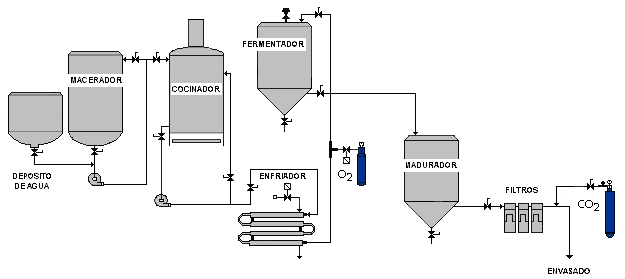
\includegraphics[scale=0.7]{procDeFab.jpg}}
		\caption{Proceso productivo para elaboración de cerveza}
	    \label{ProcFab}
	\end{figure}
	
	\par
	De todas las etapas antes mencionadas, el macerado es el proceso que reviste interés en este proyecto, ya que durante este el preparado es susceptible a modificaciones de manera de asegurar el resultado deseado. Como explica \cite{Papazian} “El proceso es continuado durante un período de tiempo con ajustes controlados de las temperaturas y pH que activa diferentes enzimas para descomponer los almidones solubles y las proteínas”. Estos ajustes requieren de una atención intensiva durante el proceso por parte del productor, y por tanto, la mayoría de estos no llevan a cabo estas prácticas. Los productores usualmente emplean una única medición de temperatura y pH realizada al inicio del proceso, involucrando en este momento todos los ajustes necesarios y presumiendo que estos valores no se modificaran durante el resto de la maceración.
	\par
	La activación de enzimas presentes en la malta toma un papel protagonista durante el proceso de maceración. El hecho de que las mismas se activen y el grado en el que lo hacen determina el nivel de aprovechamiento de la materia prima utilizada. La calidad del mosto resultante se mide en relación a la densidad del mismo al final del proceso. Cada receta de cerveza conlleva un valor de densidad a ser obtenida, desvíos por encima o por debajo devienen en malos resultados del proceso. Esta densidad objetivo determina la cantidad de insumos (kilogramos de malta) a ser utilizados. Por tanto, realizar un correcto monitoreo del proceso, buscando de esta manera asegurar las condiciones dentro de las cuales las enzimas son activadas es vital para el cumplimiento de los objetivos del proceso de maceración.
	\par
	Otro factor determinante en el resultado de densidad, proviene del cálculo de la cantidad de insumos a ser utilizados. En este cálculo, es utilizado un valor que representa la capacidad que tiene el equipo de producción (tanques maceradores) para extraer los subproductos de la malta de forma de cumplir el objetivo de densidad para el proceso. Los productores utilizan un valor genérico para este cálculo, no realizando así el correspondiente ajuste a las características de su equipo. En forma consecuente, los valores obtenidos del cálculo de insumos se alejan de la cantidad necesaria a ser utilizada para un equipo específico.
	\par
    Dentro de este contexto, se propuso el desarrollo de un prototipo de hardware y software para asistir al productor de cerveza artesanal en el proceso de maceración a través de la planificación de procesos, monitoreo de variables mediante sensores, estimación de variables de control y análisis intensivo de variables intervinientes y sus relaciones.
    \par
    Esta herramienta brinda al productor facilidad para realizar el seguimiento de la evolución del proceso, permitiendo identificar los momentos apropiados donde realizar acciones correctivas. Comportándose las variables (pH y temperatura) según lo esperado en los distintos períodos de la maceración, se evitan resultados disímiles entre diferentes maceraciones y se optimiza la utilización de la malta a través del control puntual de las actividades enzimáticas, derivando en una disminución de insumos y costos.
    \par
    De forma adicional, el sistema provee la capacidad de calcular un valor ajustado, con cada experimento de maceración, de la cantidad de insumos necesaria a ser utilizada para una receta particular. Este ajuste es realizado a partir de un cálculo, repetido en cada experimento de maceración, mediante el cual se obtiene el rendimiento del equipo.
    
\section{Estado del arte}
    \par
    Las herramientas existentes asisten en el seguimiento de todo el proceso de fabricación siendo las más reconocidas Brew-o-matic\textsuperscript{®}\footnote{\url{http://www.brew-o-matic.com.ar}}, BeerSmith\textsuperscript{®}\footnote{\url{http://beersmith.com}} y BrewersFriend\textsuperscript{®} \footnote{\url{https://www.brewersfriend.com}}. Algunas de estas herramientas de software presentan integraciones con productos de hardware para la recolección de mediciones mediante sensores, aunque solo se enfocan en la etapa de fermentación. El paquete de sensores más comúnmente utilizados por los software es Tilt®\footnote{\url{https://tilthydrometer.com/}}. Para su funcionamiento, estas herramientas requieren, en forma indistinta, el ingreso manual de los datos o variables intervinientes en forma muy detallada (tipo y marca de la malta, pH y concentración de sedimento del agua, temperaturas, tiempos, etc). Con los datos ingresados y, mediante ecuaciones, heurísticas y características de los insumos las herramientas pueden estimar las variables de control (densidad, volumen, etc). Mediante las variables obtenidas, el cervecero puede verificar que el proceso se comporta según lo esperado. Como se mencionó antes, los cálculos sin ajuste del rendimiento del equipo producen resultados que difieren de los reales, por tanto estas herramientas resultan poco efectivas para el control de los procesos. Además, ninguna profundiza el proceso de maceración, sólo ofrecen el cálculo de rendimiento y de insumos en base a la teoría y para infusiones simples.

\section{Objetivos}
\label{secccionObjetivos}
    \par
    A continuación se presentan los objetivos para el desarrollo de este proyecto.

    \subsection{Objetivos generales}
        \par
        Desarrollar un prototipo de hardware y software para asistir al productor de cerveza artesanal en la planificación, seguimiento y evaluación del proceso maceración. 
    \subsection{Objetivos específicos}
        \begin{itemize}
            \item Analizar, diseñar y construir un sistema electrónico para la medición mediante el sensado de las variables intervinientes en el proceso de maceración.
            
            \item Desarrollar una aplicación móvil que brinde funcionalidades que faciliten la planificación, seguimiento y evaluación del proceso de maceración.
            
            \item Analizar, desarrollar, aplicar y utilizar una interfaz como medio de comunicación entre el sistema electrónico y la aplicación móvil.
            
            \item Ensamblar y validar el prototipo como una construcción del sistema electrónico, la aplicación móvil y la interfaz.
        \end{itemize}
 
\section{Alcance}
    \par
    En este apartado se presenta el alcance del proyecto el cual fue definido en etapas previas\footnote{Este alcance fue definido en el documento de Anteproyecto} al desarrollo del presente proyecto. El cual incorpora, las inclusiones, exclusiones y supuestos que fueron considerados.
    \par
    Se desarrollará un prototipo de hardware y software compuesto por un sistema electrónico y una aplicación móvil. El primero estará formado por un conjunto de sensores ubicados en diferentes puntos que medirán los valores de temperatura y pH del preparado. Por otra parte, un controlador transmitirá a través de una interfaz los valores sensados. La aplicación, por su parte, se encargará de brindar las funciones de planeamiento de procesos de maceración, simples y complejos, incorporando estimación de variables de control, configuración de estrategias de obtención, monitoreo y notificación de desvíos de medidas, registro histórico de procesos, visualización gráfica, análisis estadístico y comparativo de la evolución temporal de variables intervinientes en diferentes maceraciones a partir de muestras puntuales, medidas representativas o valores ingresados.
    \par
    El sistema será desarrollado para un usuario con conocimientos teóricos suficientes que pueda entender y relacionar la información presentada, y reaccionar en consecuencia si el proceso lo requiere. El usuario será responsable del ingreso manual de datos de insumos, medidas de densidad, y comienzo y fin del proceso en la aplicación móvil.
    \par
    El desarrollo no proveerá un sistema automatizado de macerado ni una planificación, seguimiento y evaluación del proceso, sino que proveerá datos útiles y fidedignos a través de sus funcionalidades para asistir en dichas actividades. El prototipo propuesto será funcional, cumplirá las características previamente mencionadas sin alcanzar la etapa de implementación.
    \par
    Se da por aceptado que el dispositivo móvil cuenta con los servicios Wi-Fi y Bluetooth funcionando en forma correcta y operando con una versión actual del sistema operativo o de no más de un año de antigüedad en relación a la fecha de este desarrollo. En caso de utilizar conexión Wi-Fi para la interfaz, se deberá disponer de un dispositivo de red Router para el establecimiento de una red local y se configurarán los parámetros de red del sistema electrónico en forma manual.
    \par
    La precisión de los valores medidos difiere según la calidad de los sensores. Como se propone el desarrollo de un prototipo, los mismos pueden no ser exactos y no se realizará un análisis en profundidad en relación a este nivel de precisión. 
    \par
    Se deja para un futuro desarrollo la posibilidad de supervisar múltiples maceradores simultáneamente. 
 
\section{Metodología}

    \par
    En este apartado se presenta la metodología utilizada para el desarrollo del presente proyecto.
    \par La metodología seleccionada para este proyecto es la de ciclo de vida en cascada enmarcando el desarrollo completo del sistema. En el mismo, cada proceso es secuencial y la finalización de uno de ellos es el punto de inicio del siguiente.
    
    \par Al finalizar cada etapa se presenta un hito, que es el resultado de la etapa, el cual está sujeto a determinados criterios de aceptación. En cada etapa, el director del proyecto es quien juzga si los resultados que obtenidos satisfacen estos criterios.

    \paragraph{Etapas:}
        \begin{enumerate}
            \item Análisis temático y de requerimientos:
                \par En la etapa inicial se realiza una investigación bibliográfica, enfocada en el estudio del procedimiento de fabricación de cerveza artesanal, con especial atención en los procesos y subprocesos del macerado. Se redacta en forma adicional un análisis de requerimientos para el proyecto. Al finalizar esta etapa se documenta el Análisis temático que contendrá las bases teóricas que sustentan este proyecto.
                \par \textit{Hito 1: Adquisición de conocimientos necesarios.}
                
            \item Análisis, diseño y desarrollo del componente Hardware:
                \par Se lleva a cabo una investigación y análisis de potenciales soluciones para el abordaje del hardware, luego se  documenta esta investigación y se justifica la elección de la solución. Luego, se realiza un aprendizaje de desarrollo de la tecnología utilizada en la solución, para en forma consecuente, realizar el diseño y desarrollo de este sistema.
                \par \textit{Hito 2: Sistema electrónico desarrollado.} 
                
            \item Análisis, diseño y desarrollo del componente Software:
                \par En esta etapa, se realiza una investigación y análisis de potenciales tecnologías móviles a utilizar que son documentadas junto a la elección de mayor conveniencia para esta etapa. A continuación, se lleva a cabo un aprendizaje de desarrollo de aplicaciones en esta tecnología, para en forma consecuente, producir el diseño y desarrollo de la aplicación.
                \par \textit{Hito 3: Aplicación móvil desarrollada.}
                
            \item Análisis, diseño y desarrollo de la Interfaz Hardware - Software:
                \par Se entiende la interfaz como un espacio, lugar donde se desarrolla la interacción y el intercambio entre dos sistemas. Disponiendo del sistema de hardware y la aplicación móvil, se realiza una investigación y análisis de posibles alternativas, procediendo a continuación con el desarrollo de la misma.
                \par \textit{Hito 4: Interfaz desarrollada.}
                
            \item Integración y ciclo de pruebas:
                \par Se realiza la integración de los desarrollos y un ciclo de pruebas de campo para corroborar el correcto funcionamiento del sistema. Por último, se concreta con la redacción del informe final del proyecto.
                \par \textit{Hito 5: Proyecto Finalizado.}

        \end{enumerate}